\section{Day 1: Welcome, Intro to Java and Git (Sept 4, 2025)}

Contrary to CSC110 and CSC111, this course isn't that big on theory. You can do well here even if you didn't do stellar previously. We are tackling a different side of computer science here.

This course is team based, and consists of 6 modules, and is mainly about Java, although the first module is a little different and you'll learn what Git is.\footnote{i need to learn what git is fr, like don't look at the commit history of this repo plsplsplspls}

\subsection{The Software Lifecycle}
\begin{enumerate}
\item Planning and analysis
\item Define requirements
\item UI and UX design
\item Design and develop the code
\item Testing and verification
\item Deployment
\item Maintenance
\end{enumerate}
Every project has a \textbf{client}, who pays the team to build some software. Teams are led by a \textbf{manager} overseeing the entire thing, with subordinates who are responsible for their own respective bits and pieces of the product. The client usually provides the specifications and desired feature-set. The \textbf{UI/UX designer} creates and designs the interface and experience, while the \textbf{software team} develops the actual product. Sometimes there is a separate \textbf{quality assurance} (QA) division who runs tests and verifications, but the dev team can be involved too. The \textbf{DevOps engineer} focuses on the software development lifecycle.

In CSC301 and CSC309, you will encounter and learn how to interact with a real client. Most requests are handled through a \textit{ticket system}, where tickets made can be bug reports, feature requests, or something else entirely. Maintenance is an ongoing process, expect to deal with a lot of tickets if you plan on doing SWE!

\subsection{Design Ideas}
\begin{itemize}
\item having a running program be a network of objects: layers are separated cleanly to facilitate development, testing, and maintenance. want `loose coupling, high cohesion', avoiding spaghetti code
\item each object should be specialized and specific: code for a use case interaction should be separate from all other code
\end{itemize}

\subsection{Team Based Learning Principles}
Individual readiness assurance tests (iRATs) and team readiness assurance tests (tRATs) are multiple choice tests that will be administered starting week 2.

Teams come up with more ideas than individuals do. Rely on and trust your teammates. Identify each others' strengths and put them to use.

\subsection{Learning Java: public static void main(String[] args)}
Here are some things you should know from your first year courses:

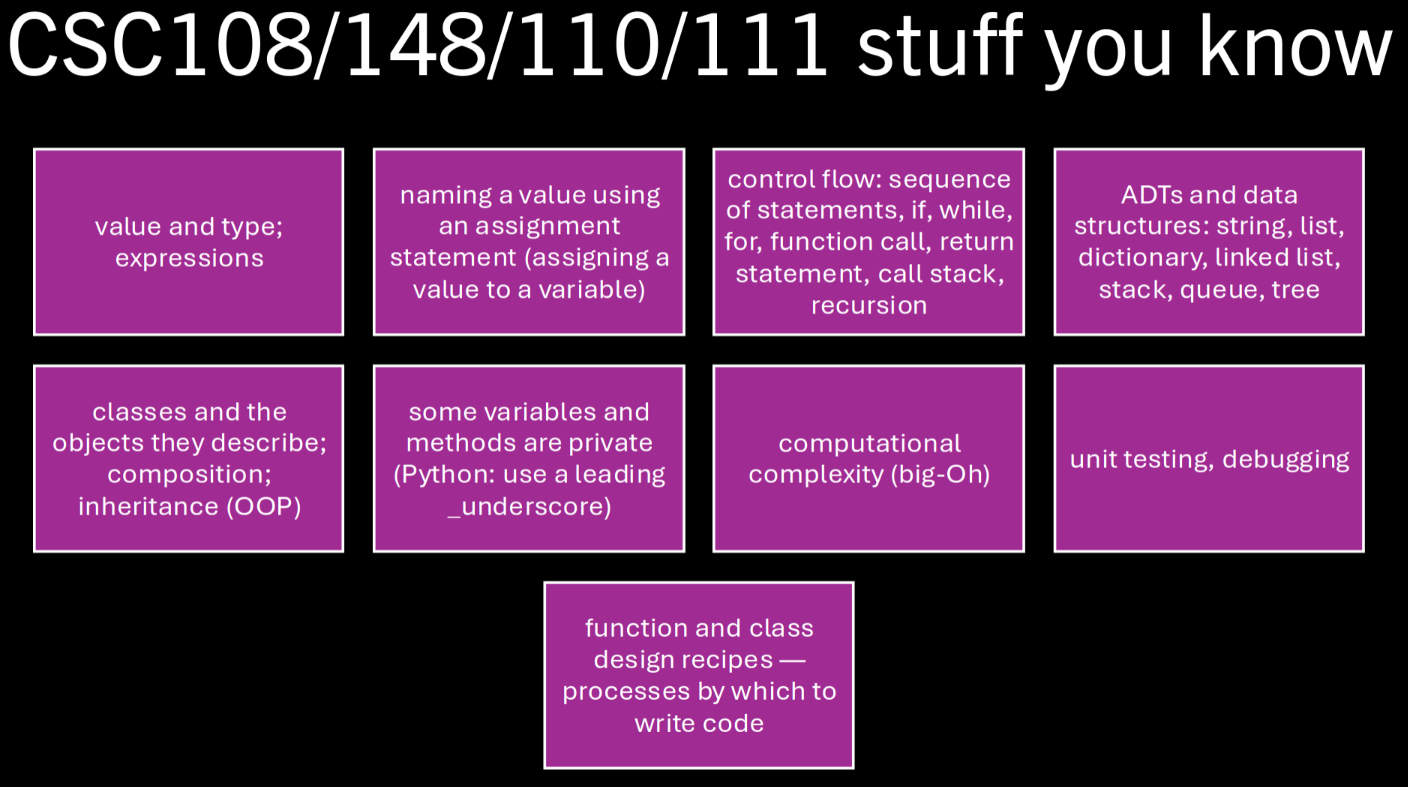
\includegraphics{csc207/figures/review.jpg}

\noindent Now we will look at `Hello, World!' in Java.

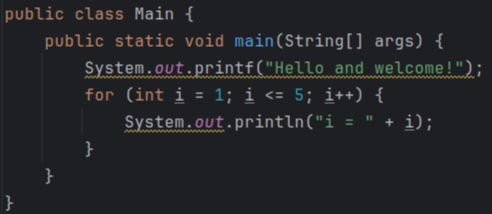
\includegraphics{csc207/figures/helloworld.jpg}

\begin{description}
    \item[public] All code (with some exceptions) call call this method\footnote{the opposite of this is \textbf{private}, where only code in the current class can call this method}
    \item[static] Static means this is a top level function, you don't need to create an object in order to call it
    \item[void] Void means that there is no return value
    \item[main] The name of the method, is the entry point of the program
    \item[String{[]}] An array of strings
\end{description}

Note that there are a lot more words in Java than Python!

In Java, \texttt{System.out} is an instance of the \texttt{PrintStream} object. We call \texttt{printf} and a variety of similar methods on \texttt{System.out} to perform I/O. Note that for loops look different than in Python, but we didn't discuss them in depth today.

GitHub contains repositories, which are projects that people have created. We can clone repositories through IntelliJ IDEA: Select File, New, then Project from Version control. By doing this you have a copy of everything in the original repo.

We will learn more about git soon, but the professor did talk about Git quite a bit today and mentioned words like commit, branch, merge, push, etc. The following remark is just for completeness.

\begin{remark}[On Git]
After you commit your changes to a project locally, you can then push them to a more central location such that others can pull them to download to their machines. A commit is like a snapshot of the project at a specific time. When cloning a repo, your cloned project inherits all of the git commit history. The history resembles a tree-ish structure, where when a developer wants to add something, they create a branch to work separately. To have their work enter the `main body' again they would merge their branch. We will get into the complex merging techniques later.
\end{remark}

For inheritance in Java, instead of typing \texttt{class Student(Person)} like in Python, you would write \texttt{public class Student extends Person} or \texttt{public class Student implements Person} depending on the context.

Note that in Java, Strings are immutable. When you use $+$ on two strings, you are creating a new string entirely which incurs a lot of overhead. Instead, use a \texttt{StringBuilder} or \texttt{.append} to concatenate/build strings.

In this course, we \textbf{like} creating helper methods. IntelliJ helps in the creation of helper methods, and renaming variables. Learning these tools will help you save development time.

Next week, you need a device that can access Quercus since you will need to complete an iRAT and tRAT.
